\documentclass[a4paper,12pt]{article}
	\usepackage{graphicx}
	\usepackage[utf8]{inputenc}
	\usepackage[T1]{fontenc}
	\usepackage{listings}
	\usepackage{color}
	\usepackage{amsmath}

	\definecolor{dkgreen}{rgb}{0,0.6,0}
	\definecolor{gray}{rgb}{0.5,0.5,0.5}
	\definecolor{mauve}{rgb}{0.58,0,0.82}

	\lstset{frame=tb,
	  language=Python,
	  aboveskip=3mm,
	  belowskip=3mm,
	  showstringspaces=false,
	  columns=flexible,
	  basicstyle={\small\ttfamily},
	  numbers=none,
	  numberstyle=\tiny\color{gray},
	  keywordstyle=\color{blue},
	  commentstyle=\color{dkgreen},
	  stringstyle=\color{mauve},
	  breaklines=true,
	  breakatwhitespace=true
	  tabsize=3
	}
	\title{ Mecânica Clássica I}
	\author{\small André Del Bianco Giuffrida\\ \small IFSC - USP\\ \small andre.giuffrida@usp.br}
	\date{}
\begin{document}
\maketitle
	A força $F(t) = F_0 (1-e^{-a t})$ age sobre um oscilador harmônico que está em repouso com massa $m$ onde $k=4ma^2$ e $b = ma$.
	
	Escrevendo a equação diferencial temos:
	
	\[ \ddot{x} + a\dot{x} + 4a^2 x = \frac{F_0}{m} (1-e^{-a t}) \]
	
	Aqui temos uma Equação diferencial não homogênea, irei resolver numéricamente esta equação utilizando o método de euler para discretizar o problema.
	\[ \dot{x} = \frac{dx}{dt} = \frac{ x_{i+1} - x_{i} }{dt} \]
	\[ \ddot{x} = \frac{d\dot{x}}{dt} = \frac{ \dot{x}_{i+1} - \dot{x}_{i} }{dt} \]
	e assim conseguimos escrever a equação toda em termos de $x_i$ , $t$ e $dt$
	onde $dt$ aqui é discreto
	\[ \frac{ x_{i+2} - 2x_{i+1}- x_{i} }{dt^2} + a\frac{ x_{i+1} - x_{i} }{dt} + 4a^2 x_{i} = \frac{F_0}{m} (1-e^{-a t}) \]
	
	\[ x_{i+2} \Big(\frac{ 1 - 2x_{i+1}- x_{i} }{dt^2} \Big) + a\frac{ x_{i+1} - x_{i} }{dt} + 4a^2 x_{i}  = \frac{F_0}{m} (1-e^{-a t}) \]
	
	\[ x_{i+2} = \frac{\frac{F_0}{m} (1-e^{-a t})dt^2 - a (x_{i+1} - x_{i}) dt -  4a^2 x_{i} dt^2}{1 - 2x_{i+1}- x_{i}}\]


	
	\begin{figure}[h]
		\centering
		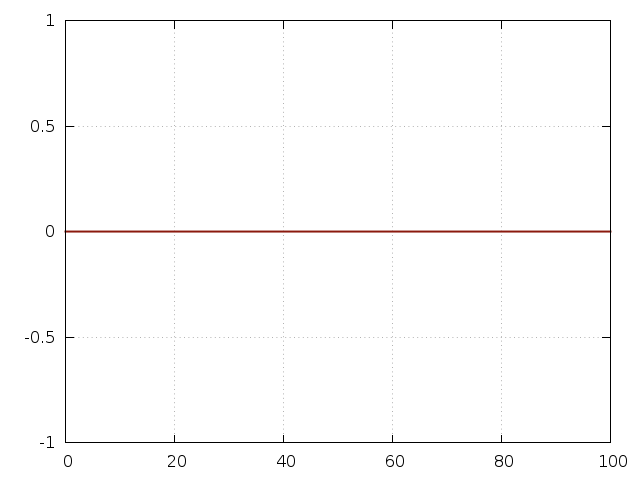
\includegraphics[scale=0.6]{10o0.png}
		\caption{None}
	\end{figure}
	
	\end{document}
	
